\documentclass{beamer} 

\usepackage[utf8]{inputenc}
\usepackage{graphicx}
\usepackage{multicol}
\usepackage{listings}
\usepackage{pdfpages}


\begin{document}

\title{Using formalism to design secure systems}
\author{Stefan Nožinić (stefan@lugons.org)}

\frame{
\titlepage
}

% https://pdfs.semanticscholar.org/5b26/c71affdd6db82e58344510512d6a2c9f070a.pdf
% https://etd.ohiolink.edu/apexprod/rws_etd/send_file/send?accession=ucin1623169331790079&disposition=inline
% https://www.dsn.kastel.kit.edu/publications/2022-PCN-TLA+.pdf
% https://users.cs.northwestern.edu/~ychen/Papers/Narayana-wimax.pdf
\begin{frame}
    \frametitle{Agenda}
    \begin{itemize}
        \item What are formal methods
        \item How to formalize systems 
        \item Several examples from literature 
        \item One real world example
        \item Conclusion
    \end{itemize}

\end{frame}

\begin{frame}[fragile]
	\begin{lstlisting}[language=C++]

int main() {
    int i = readInteger();
    i++;
    return 0;
}

	\end{lstlisting}
	
\end{frame}

\begin{frame}
    \begin{center}
        \LARGE{\textbf{How to model this simple program formally as state machine?}}
    \end{center}

\end{frame}


\begin{frame}[fragile]
    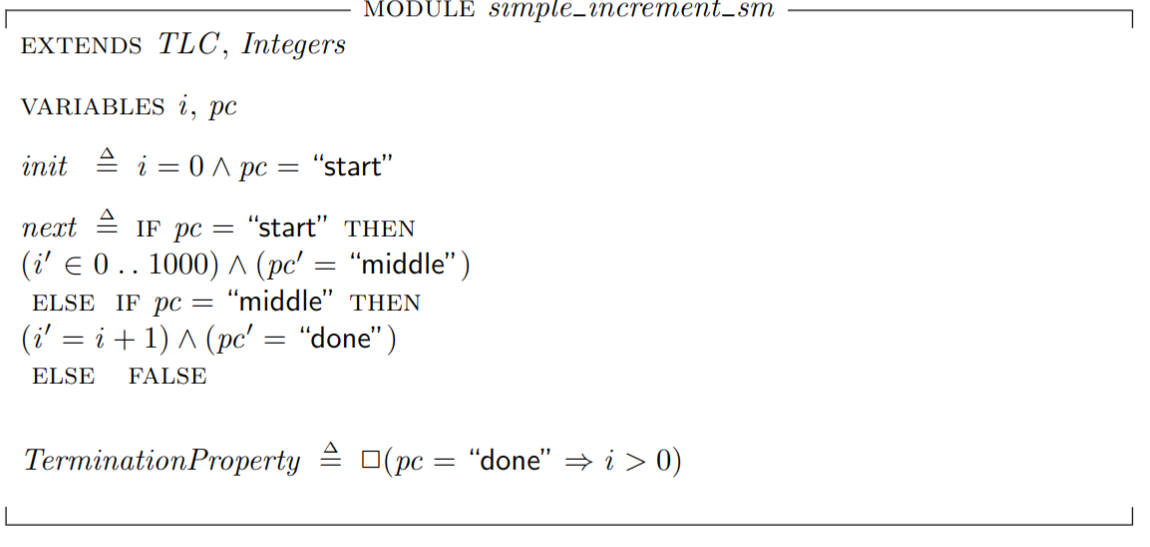
\includegraphics[width=\textwidth]{./sm_increment.png}
\end{frame}

\begin{frame}
    \begin{center}
        \LARGE{\textbf{Two-phase commit}}
    \end{center}
\end{frame}

\begin{frame}[fragile]
    \begin{lstlisting}
---- MODULE twoPhase ----
EXTENDS TLC

CONSTANT RM 
VARIABLE rmState 
VARIABLES tmState, tmPrepared, msgs 

Messages == [type : {"prepared"}, rm : RM] \cup 
    [type : {"commit", "abort"}]



TPTypeOK == 
    /\ rmState \in [RM -> {"working", "prepared", 
        "committed", "aborted"}]
    /\ tmState \in {"init", "done"}
    /\ tmPrepared \subseteq RM
    /\ msgs \subseteq Messages


    \end{lstlisting}
\end{frame}

\begin{frame}[fragile]
    \begin{lstlisting}
TPInit == 
    /\ rmState = [r \in RM |-> "working"]
    /\ tmState = "init"
    /\ tmPrepared = {}
    /\ msgs = {}

    \end{lstlisting}
\end{frame}



\begin{frame}[fragile]
    \begin{lstlisting}

TPNext ==
    \/ TMAbort
    \/ TMCommit
    \/ (\E r \in RM : RMPrepare(r))
    \/ (\E r \in RM : RMChoosetoAbort(r))
    \/ (\E r \in RM : TPRecvPrepared(r))
    \/ (\E r \in RM : RMChooseToCommit(r))
    \/ \E r \in RM : RMAbort(r)



====
    \end{lstlisting}


\end{frame}


\begin{frame}[fragile]
    \begin{lstlisting}



TPRecvPrepared(r) == 
    /\ tmState = "init"
    /\ [type |-> "prepared", rm |-> r] \in msgs
    /\ tmPrepared' = tmPrepared \cup {r}
    /\ UNCHANGED << tmState, msgs, rmState >>
        
    \end{lstlisting}


\end{frame}

\begin{frame}[fragile]
    \begin{lstlisting}
TMCommit == 
    /\ tmState = "init"
    /\ \A r \in RM : r \in tmPrepared
    /\ msgs' = msgs \cup {[type |-> "commit"]}
    /\ tmState' = "done"
    /\ UNCHANGED <<rmState, tmPrepared >> 
    
TMAbort ==
    /\ tmState = "init"
    /\ tmState' = "done"
    /\ \E r \in RM : rmState[r] = "aborted"
    /\ msgs' = msgs \cup {[type |-> "abort"]}
    /\ tmPrepared' = {} 
    /\ UNCHANGED  <<rmState>>


    \end{lstlisting}
\end{frame}


\begin{frame}[fragile]
    \begin{lstlisting}
RMPrepare(r) == 
    /\ rmState[r] = "working"
    /\ msgs' = msgs \cup 
        {[rm |-> r, type |-> "prepared"]}
    /\ rmState' = [rmState 
        EXCEPT ![r] = "prepared"]
    /\ UNCHANGED <<tmPrepared, tmState>>

RMAbort(r) == 
    /\ rmState[r] = "working"
    /\ rmState' = [rmState 
        EXCEPT ![r] = "aborted"]
    /\ UNCHANGED 
        <<tmPrepared, tmState, msgs>>

    \end{lstlisting}
\end{frame}

\begin{frame}[fragile]
    \begin{lstlisting}
RMChoosetoAbort(r) == 
    /\ rmState[r] = "working"
    /\ [type |-> "abort"] \in msgs 
    /\ rmState' = [rmState 
        EXCEPT  ![r] = "aborted"]
    /\ UNCHANGED  
        <<tmState, tmPrepared, msgs>>


    \end{lstlisting}

\end{frame}

\begin{frame}[fragile]
    \begin{lstlisting}
RMChooseToCommit(r) == 
    /\ rmState[r] = "working"
    /\ [type |-> "commit"] \in msgs 
    /\ rmState' = [rmState 
        EXCEPT  ![r] = "committed"]
    /\ UNCHANGED  
        <<tmState, tmPrepared, msgs>>




====
    \end{lstlisting}


\end{frame}

\begin{frame}
    \frametitle{PlusCal}
    \begin{itemize}
        \item A little more progreammer-friendly 
        \item We specify processes and TLC will check all behaviours
    \end{itemize}
\end{frame}

\begin{frame}[fragile]
    \frametitle{Simple clock}
    \begin{itemize}
        \item We start from anywhere between 1 and 12 (including 1 and 12)
        \item in every iteration, we increase by one 
        \item when we reach 12, we reset back to 1 
        \item We also state that "x will be eventually one"
    \end{itemize}
\end{frame}



\begin{frame}[fragile]
    \frametitle{Real world example - health monitor}
    \begin{itemize}
        \item We have several nodes (lets say nodes are 1, 2 and 3)
        \item Every node can reboot and recover later on 
        \item Every node has one instance of service called "replicator"
        \item When node is down, its replicator instance gets transferred to another node which is up 
        \item When we detect that replicato instance is stuck, we kill it and restart it 
        \item We state that eventually if replicator is stuck, this will lead to either it being killed or recovered by itself
    \end{itemize}
\end{frame}

\begin{frame}
    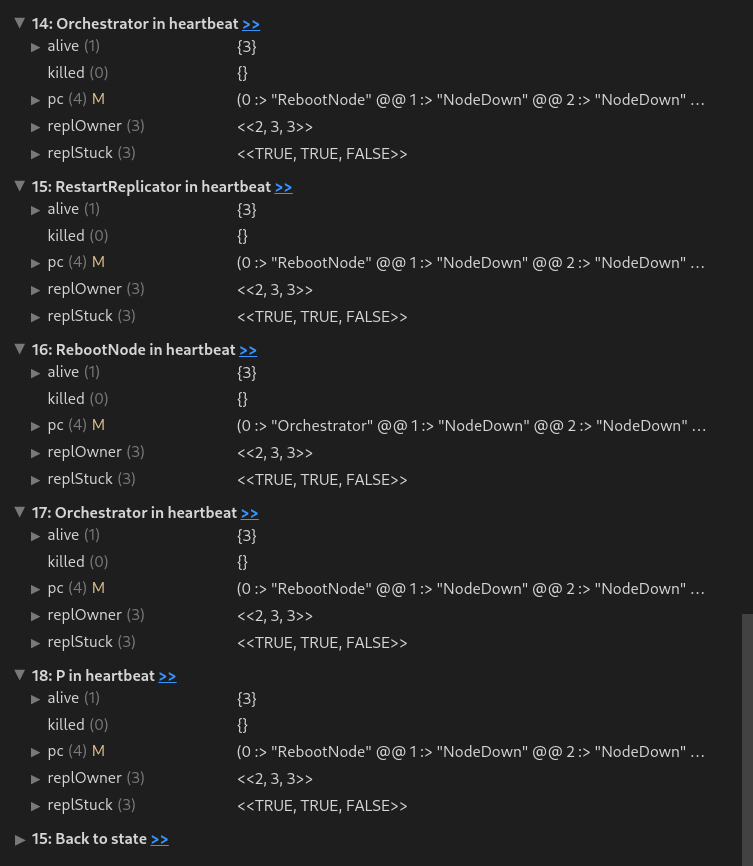
\includegraphics[width=0.9\textwidth, height=0.9\textheight]{examples/img1.png}
\end{frame}


\begin{frame}
    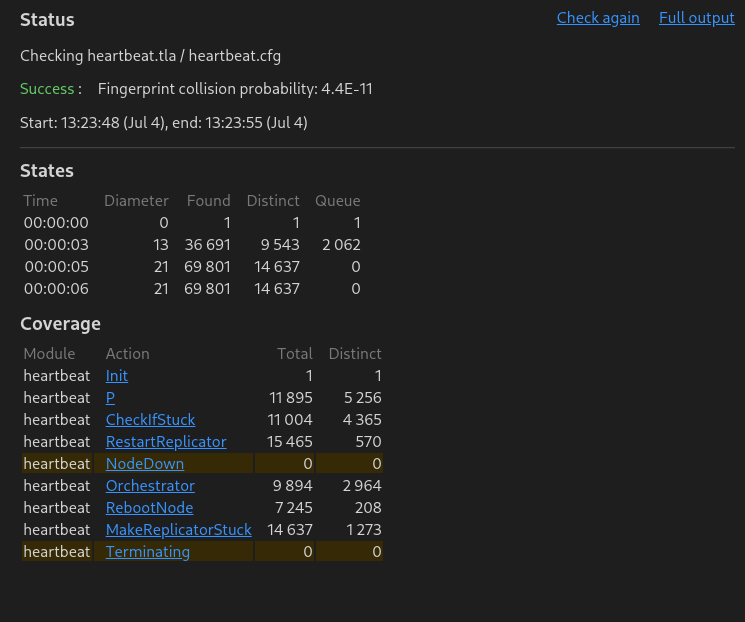
\includegraphics[width=0.9\textwidth, height=0.9\textheight]{examples/img2.png}
\end{frame}
\end{document}
